\addcontentsline{toc}{chapter}{Messdaten} % damit trotzdem im Inhaltsverzeichnis
\label{Protokoll}


% \thispagestyle{empty}

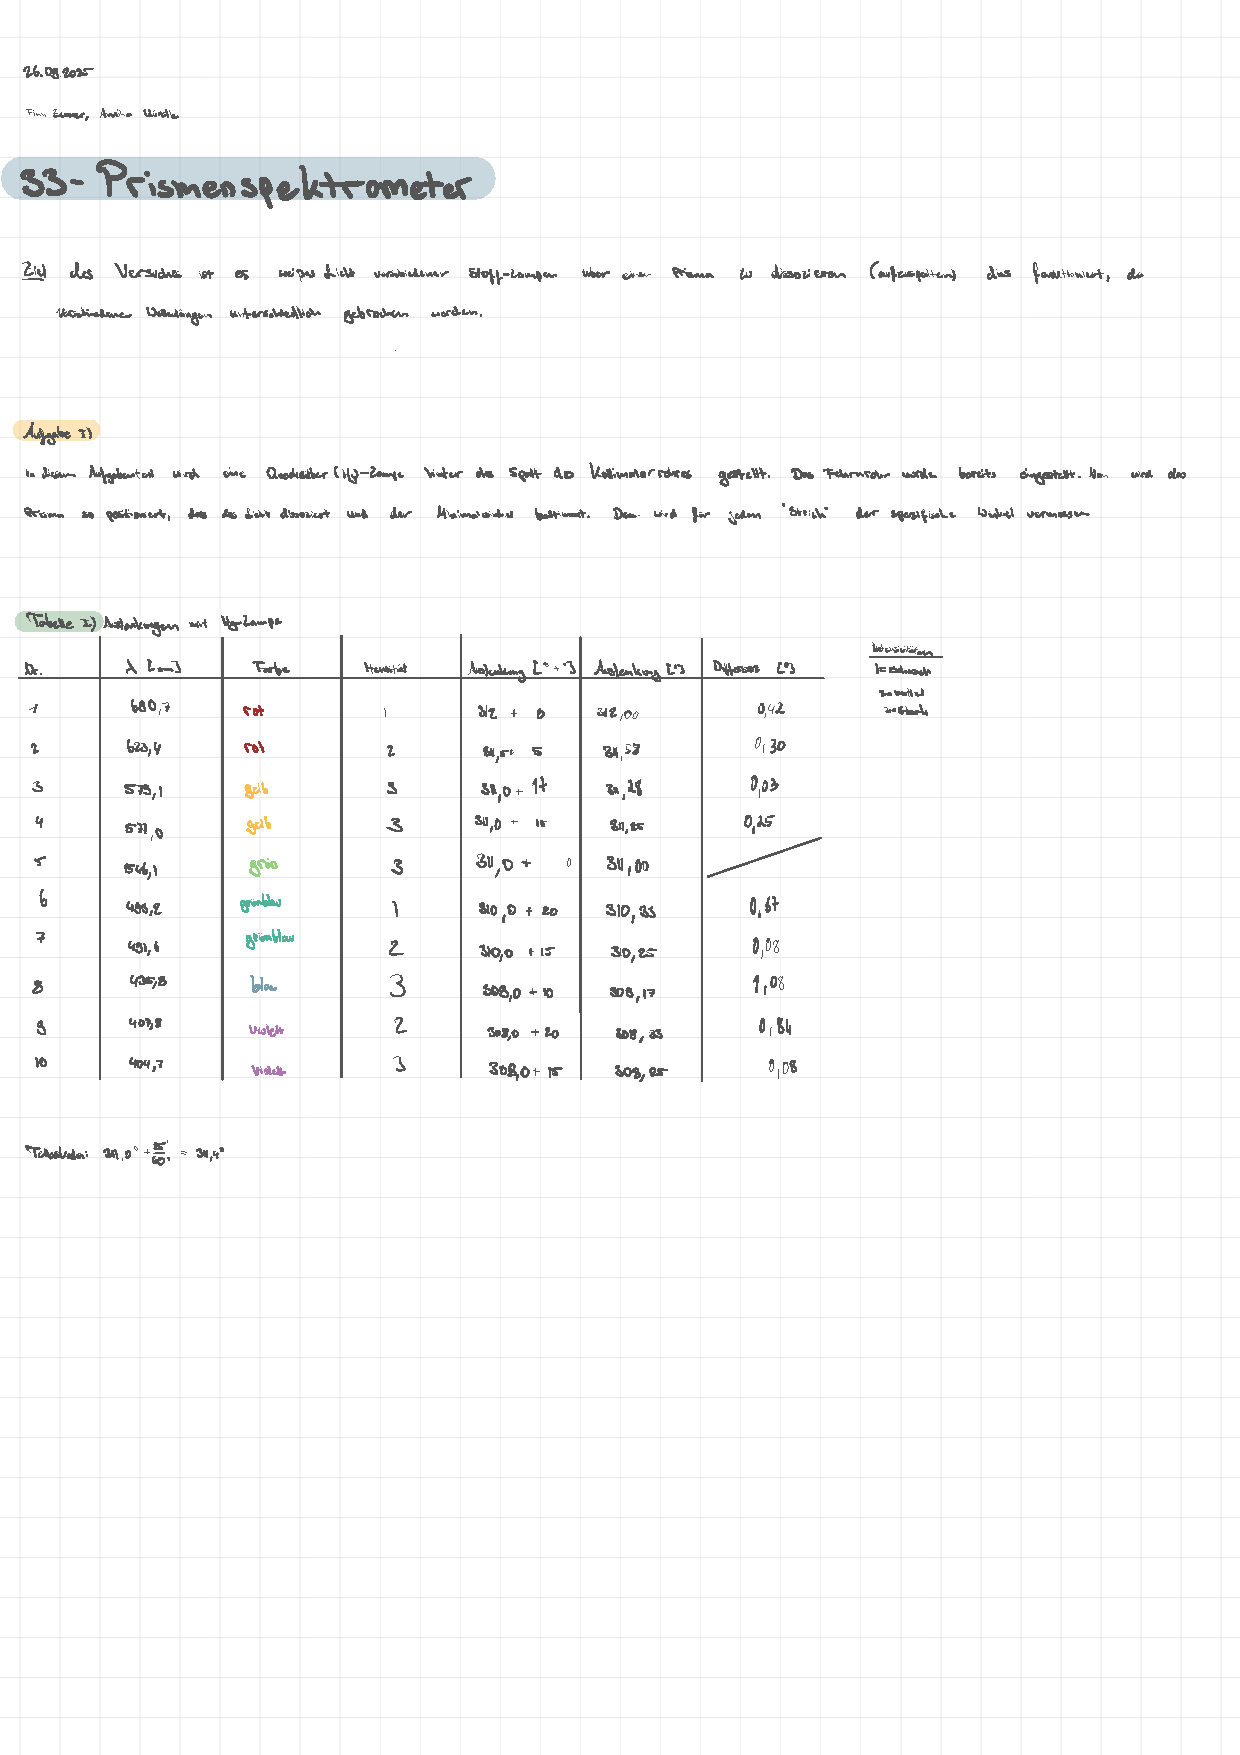
\includepdf[
  pages=1-2,               
  pagecommand={\thispagestyle{empty}} 
]{Protokolle/\versuchsnummer/Chapter/Messprotokoll.pdf}



\addcontentsline{lot}{table}{\protect\numberline{\thechapter.1} Auslenkung mit Quecksilberlampe}
\addcontentsline{lot}{table}{\protect\numberline{\thechapter.2} Auslenkung mit Heliumlampe}
\addcontentsline{lot}{table}{\protect\numberline{\thechapter.3} Auslenkung mit Wasserstofflampe}
